\section{Post-Training}
\label{sec:alignment}
In comparison to Nemotron Nano 2, we significantly scale up the compute in post-training for \ourmodel. 
% In total, post-training stage consumes \todo{BB} percent of total training compute for \ourmodel.
Noticeably \ourmodel is our first effort to scale up reinforcement learning (RL) in the post-training stage. 
% Specifically, reinforcement learning consumes \todo{CC} percent of the total training compute. 
This RL scale up is empowered by multi-environment reinforcement learning (discussed in Sections \ref{subsec:SFT} to \ref{subsec:RLHF}), where we train on all environments simultaneously for the first time. We adopted Nemo-Gym, a RL training environment orchestration framework with a large collection of RL environments; this is integrated with Nemo-RL as the RL training framework as discussed in Section \ref{subsubsection:RLinfra} \citep{nemo-gym, nemo-rl}. We open source Nemo-Gym and Nemo-RL to enable the broader community to facilitate large-scale RL training, as well as collaborative and distributed RL environment building.

In the rest of this section, we discuss the post-training methodology for \ourmodel, which includes supervised finetuning (SFT) in \S\ref{subsec:SFT}, multi-environment reinforcement learning in \S\ref{subsec:RLVR}, and reinforcement learning from human feedback (RLHF) in \S\ref{subsec:RLHF}. The final evaluation results can be found in \S\ref{subsec:final_model_evals}. Our post-training methodology results in best-in-class performance in a variety of reasoning and agentic tasks, along with token efficiency, reasoning on/off control, reasoning budget control, and tool-integrated reasoning capabilities.  

\subsection{Supervised Fine Tuning}
\label{subsec:SFT}
Since the release of Nemotron 2 Nano, we have significantly improved our SFT strategy. We increased dataset quality and diversity, adding a wide variety of new data with an emphasis on multi-step and multi-turn agentic tasks. Different from the SFT data in the pre-training stage, the SFT stage data is more focused on agentic tasks and has the chat-template applied. We release the majority of our training data and open source our SFT codebase.

\subsubsection{Chat Template}
We allow using \ourmodel in reasoning or non-reasoning mode through the chat template. 
% In reasoning mode, the chat template prepends the think token with a new line to signal the model to reason, while in non-reasoning mode the chat template prepends the think token and closing think token. This allows for the model to 

In reasoning mode, we alter the reasoning flow for the following conversation scenarios:
\begin{itemize}
    \item \textit{Multi-Step}: In a series of assistant model calls, the existing reasoning tokens are preserved to allow the model to re-use existing reasoning for subsequent step.
    \item \textit{Multi-Turn}: When a user message is introduced, any reasoning from previous turns are dropped.
\end{itemize}

For tool calling, we use XML-style special tags to reduce character escaping, following the observations of GLM-4.5 \citep{5team2025glm45agenticreasoningcoding} and Qwen3-Coder \citep{yang2025qwen3technicalreport}.

% \todo{Venkat: Chat-template figure. We should have a link as well to the chat template?}
% \todo{JK: I added a figure let me know if its weird + I don't think we need a link to the template}

\begin{figure}[t]
    \centering
    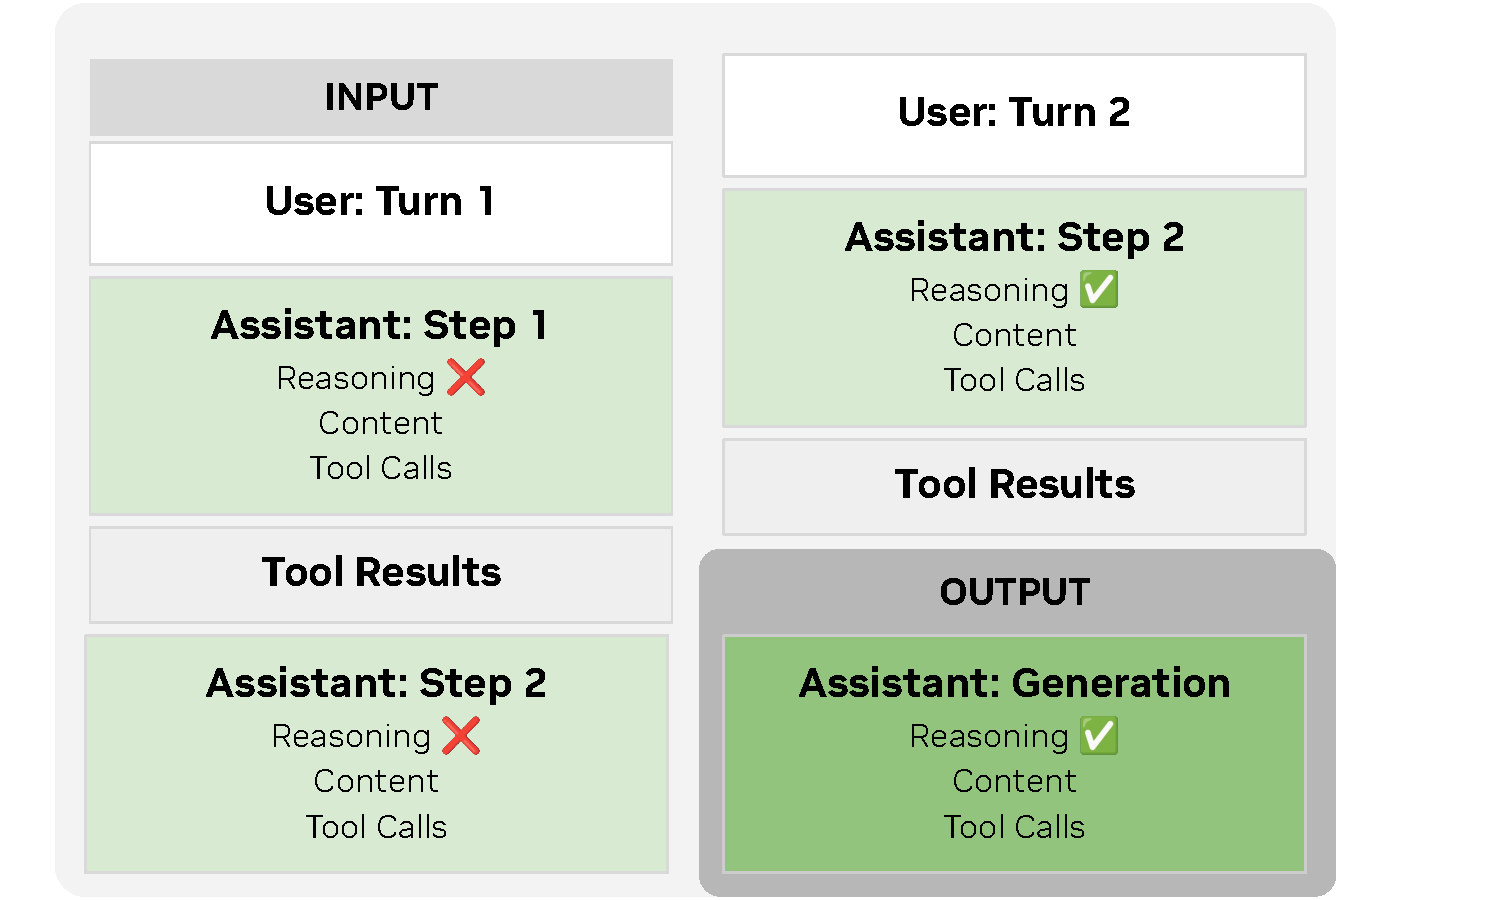
\includegraphics[width=10cm]{figures/chat_template.pdf}
    \caption{Example prompt materialization using the \ourmodel chat template for a 2-turn conversation. For a given generation, only reasoning content from the current turn is materialized into the prompt.}
    \label{fig:chat_template}
\end{figure}


\subsubsection{Data}

\textbf{Competition Math.} For math, we use a similar strategy to Nemotron Nano 2 \citep{nemotronnanov2}. However, we refresh the responses with GPT-OSS 120B \citep{openai2025gptoss120bgptoss20bmodel}. In addition, we create tool-integrated reasoning traces using Python tools and GPT-OSS 120B as the teacher model.

\textbf{Competition Code.} For code we use the same data from Nemotron Nano 2, which is made up of the prompts from \citet{ahmad2025opencodereasoning} complemented with responses from DeepSeek-R1-0528 \citep{deepseekai2025deepseekr1incentivizingreasoningcapability}.


\textbf{Conversational Tool Use.} We generate synthetic multi-turn trajectories to demonstrate conversational tool use. The generation of these trajectories involves a user that is given a task to accomplish, an agent that is instructed to help the user accomplish their task, and a tool execution environment, each of which is simulated by a language model. To limit the trajectories in the SFT training data to ones in which the actions of all of these entities are consistent with their goals, we employ a language model as a judge to evaluate the trajectories, and filter out trajectories for which the judge considers an action of an entity to be inconsistent with its goals. We use Qwen3-235B-A22B-Thinking-2507 \citep{yang2025qwen3technicalreport}, Qwen3-32B \citep{yang2025qwen3technicalreport}, GPT-OSS-120b \citep{openai2025gptoss120bgptoss20bmodel}, and Qwen3-235B-A22B-Instruct-2507 \citep{yang2025qwen3technicalreport} to generate data in this synthetic tool use trajectory generation pipeline.

\textbf{Long Context.} We generate synthetic data with a mean token length of 128k tokens and a maximum of 256k tokens to improve long-context performance, validated against a subset of RULER tasks.
% We generate synthetic data aiming to improve a subset of RULER tasks, with the mean token length of 128k tokens with a hard limit of 256k tokens. 
% \todo{Dima/Krishna: We can probably add more details}

\textbf{Formal Proofs.} For Lean theorem proving, we curated SFT data by first autoformalizating ~580k natural language theorems from online mathematics communities (AoPS, Math StackExchange, MathOverflow) into ~550k Lean 4 statements using an iterative refinement pipeline based on GPT-OSS-120B with backtranslation-based semantic verification. We then ran large-scale proof generation using Goedel-Prover-V2-32B with up to 4 independent attempts and 8 self-correction rounds per statement, yielding ~920k proof traces with compiler-verified solutions. After filtering, the final dataset contains ~300k examples pairing formal theorem statements with successful reasoning traces and proofs.

\textbf{Multilingual.} We generate multilingual data in a similar manner to Nemotron Nano 2 \citep{nemotronnanov2}. We used Qwen$2.5$-Instruct to translate our existing English post-training data into $5$ target languages, French, Spanish, Italian, German and Japanese. Our pipeline translates inputs line-by-line and skips non-translatable content like code, XML tags, URLs, etc. 
Following the translation of the English source text, we utilized a language identification tool \url{https://pypi.org/project/langdetect/} to filter out samples that did not predominantly consist of target language tokens. Additionally, we excluded samples containing specific failure modes where the Qwen model explicitly stated its inability to translate the source text.

Our multilingual corpus was further comprised of $1.62$ million text translation samples, aggregated from a combination of news-commentary datasets and proprietary sources. These samples covered bidirectional translation tasks between English and the five target languages.
%For machine translation, we used the combination of TAUS and news-commentary datasets. The resulting subset contains $1.62$M samples with $162$k samples for each language direction.


\textbf{Terminal Use.} To teach \ourmodel to complete autonomous terminal-based tasks, we generate a diverse set of verifiable tasks based on Terminal Bench \citep{tbench_2025}. In particular, we adapt data from our competitive coding, competitive math, and long context datasets to terminal bench problems. We also constructed synthetic tasks requiring data analysis and file creation and operations. Additionally, we incorporated data from SWE-Smith \citep{swesmith}, which provides real-world software engineering tasks. We use 
Qwen3-Coder-480B-A35B-Instruct \citep{qwen2025qwen25technicalreport} and Kimi-K2-Instruct-0905 \citep{kimiteam2025kimik2openagentic} to generate action trajectories for each task using the Terminus-1 and Terminus-2 agents \citep{tbench_2025}.

\textbf{General Chat.} We create SFT data by generating responses to the LMSYS \citep{zheng2023judging} and WildChat datasets \citep{li2024wildchat} using GPT-OSS-120B, Qwen3-235B-A22B-Thinking-2507, and Qwen3-235B-A22B-Instruct-2507. The data is extended to multi-turn by having the same language model simulate the user and further continue the conversation.

\textbf{Instruction Following.} We create targeted instruction following data with the methodology used in Tülu 3 \citep{lambert2025tulu3pushingfrontiers}. We simulate users in a conversation using language models seeded with a user persona from Nemotron-Personas-USA \citep{nvidia/Nemotron-Personas-USA} and instructions from IFeval \citep{zhou2023instruction} and IFBench \citep{pyatkin2025generalizing} train splits. The user language model is prompted to generate precise instruction following queries for one or more turns. We then use GPT-OSS-120B, Qwen3-235B-A22B-Thinking-2507, and Qwen3-235B-A22B-Instruct-2507 to generate responses to the user queries. The generated data is first filtered to only keep samples where all turns pass the respective instruction verifier implementations in IFEval and IFBench. Further filtering is done with a language model judge to remove samples where the responses only trivially or superficially follow instructions.

\textbf{Safety.} 
We compile a diverse set of unsafe prompts sourced from the Nemotron Content Safety v2 \citep{ghosh-etal-2025-aegis2} and the Gretel Safety Alignment v1 \citep{gretelai_gretel-safety-alignment-en-v1}  datasets to target content safety risks, and Harmful Tasks \citep{hasan2024pruning} and Red-Team-2K \citep{luo2024jailbreakv_robustness} datasets to target common jailbreak techniques. This collection is further balanced with safe prompts derived from Nemotron Content Safety v2.

For supervised fine-tuning (SFT), we apply safe prompt wrappers to unsafe prompts enabling the models to learn appropriate refusal behaviors while preserving user engagement. Various refusal strategies are implemented to align with good user experience. For instance, self-harm related prompts are paired with prompt templates encouraging the use of appropriate suicide prevention helplines. A content-safety classifier is employed to filter the responses, ensuring alignment with safety objectives.



%\textbf{Translation.} 

\textbf{Software Engineering.} To train \ourmodel for autonomous software engineering capabilities including code exploration, issue reproduction and bug fixing, we curate a dataset of coding tasks derived from real-world GitHub issues. We use the issue description and containerized execution environments from SWE-Gym \citep{pan2025trainingsoftwareengineeringagents} and R2E-Gym \citep{jain2025r2egymproceduralenvironmentshybrid} datasets. We distill trajectories from three open-source agent harnesses - OpenHands \citep{wang2025openhandsopenplatformai}, SWE-Agent \citep{yang2024sweagent}, and Mini-SWE-Agent \citep{yang2024sweagent} using Qwen3-Coder-480B-A35B-Instruct  \citep{qwen2025qwen25technicalreport} as the teacher model. 

\textbf{Science.} The science dataset spans physics, chemistry, and biology, and is produced through a unified pipeline that integrates synthetic, real, and document-based seed sources. We began by curating a set of challenging seed questions derived from Nemotron Nano v2 \citep{nemotronnanov2} as well as from scientific articles contained in the pre-training corpus. In parallel, we incorporated additional scientific articles from the same corpus as a complementary reservoir of seed material. Each article was annotated with three attributes: (1) education domain based on bert-based finetuned classifier \citep{li2024datacomp}, (2) content level (ranging from elementary to graduate), and (3) fine-grained topical categories (e.g., biology, chemistry, mathematics, law). Focusing on the graduate-level subset, we indexed these documents in a vector database and used a diverse set of science-oriented query prompts to retrieve thousands of highly relevant passages. These retrieved segments served as the foundation for generating multiple-choice question (MCQ) data, which were subsequently converted into an open-ended question-answering (OpenQA) format.

All seed sources—synthetic, real, and doc-retrieved—were subsequently processed through NeMo Data Designer \citep{nemo-data-designer}. The Data Designer was used to paraphrase prompts, produce multiple format and instruction variants, and enhance robustness across prompt styles. Reasoning traces for the SFT stage were generated using tool-integrated Python reasoning traces from GPT-OSS 120B \citep{openai2025gptoss120bgptoss20bmodel}. Crucially, all generated variants underwent rigorous LLM-judge filtering, ensuring strict format compliance, intent preservation, and high-quality reasoning consistency. During the RL stage, we further introduced targeted prompt and format augmentations to reduce prompt sensitivity and improve generalization.

A subset of STEM datasets developed in this work are released in both the multiple-choice question (MCQ\footnote{\url{https://huggingface.co/datasets/nvidia/Nemotron-RL-knowledge-mcqa}}
) and open question-answering (OpenQA\footnote{\url{https://huggingface.co/datasets/nvidia/Nemotron-RL-knowledge-openqa}}
) formats to support Nano-V3 training and broader downstream research. These datasets are fully integrated into the RLVR pipeline, with both MCQ\footnote{\url{https://github.com/NVIDIA-NeMo/Gym/tree/main/resources_servers/mcqa}}
 and OpenQA\footnote{\url{https://github.com/NVIDIA-NeMo/Gym/tree/main/resources_servers/equivalence_llm_judge}}
 environments provided through NeMo Gym \citep{nemo-gym}. This unified pipeline ensures consistent quality standards and supports robust reinforcement-learning-based evaluation and training across all STEM domains.

%The science dataset spans physics, chemistry, and biology. We constructed a subset of challenging real and synthetic seed questions derived from Nemotron Nano v2 \citep{nemotronnanov2} and scientific articles from the pretraining sets. These prompts were paraphrased with NeMo Data Designer \citep{nemo-data-designer} and augmented to produce SFT training data across several prompt and format variants to improve model robustness. Crucially, all generated variations underwent rigorous LLM-judge filtering to ensure strict format compliance and intent preservation. Additional prompt and format augmentations were introduced during the RL stage to reduce prompt sensitivity. Reasoning traces for the SFT stage were generated using tool-integrated Python reasoning traces from GPT-OSS 120B \citep{openai2025gptoss120bgptoss20bmodel}.

%In addition, we incorporated scientific articles from the pre-training corpus as a complementary source of seed material. We first tagged the entire collection along three attributes: (1) educational domain \citep{li2024datacomp}, (2) content level (elementary through graduate), and (3) fine-grained topic categories (e.g., biology, chemistry, mathematics, law). Focusing on the graduate-level subset, we indexed these documents in a vector database and used questions from established STEM benchmarks as retrieval queries. For each query, we selected thousands of relevant seed chunks, which were used to generate MCQA data and subsequently converted into ShortQA format. As with our synthetic pipeline, all generated variants underwent stringent LLM-judge filtering to ensure strict format adherence and prompt robustness reduction. All STEM RL datasets developed in this work are released in both multi-choice question (MCQ\footnote{\url{https://huggingface.co/datasets/nvidia/Nemotron-RL-knowledge-mcqa}}) and open question answering (OpenQA\footnote{\url{https://huggingface.co/datasets/nvidia/Nemotron-RL-knowledge-openqa}}) formats at high quality (HQ) to nano-V3 training and downstream research. These datasets are fully integrated into the RLVR pipeline, with both MCQ\footnote{\url{https://github.com/NVIDIA-NeMo/Gym/tree/main/resources_servers/mcqa}} and OpenQA\footnote{\url{https://github.com/NVIDIA-NeMo/Gym/tree/main/resources_servers/equivalence_llm_judge}} environments made available through NeMo Gym \citep{nemo-gym}.

\textbf{GenSelect.} We improve our model’s capability as a generative reward model by training it to identify the best solution among multiple candidates, following the approach in \cite{toshniwal2025genselectgenerativeapproachbestofn}. We adapted the problems in our math and coding SFT data by generating synthetic solutions and then selection reasoning traces including their final verdicts using GPT-OSS 120B \citep{openai2025gptoss120bgptoss20bmodel} and DeepSeek-R1-0528 \citep{deepseekai2025deepseekr1incentivizingreasoningcapability}.  

\textbf{CUDA.} We collect and synthesize 21k (PyTorch, Cuda C) pairs with seeds from HuggingFace Transformers \citep{wolf-etal-2020-transformers} and KernelBook \citep{kernelbook2025}. We first parse the PyTorch code from Transformers \citep{wolf-etal-2020-transformers} and KernelBook \citep{kernelbook2025}, and then use DeepSeek-R1-0528 \citep{deepseekai2025deepseekr1incentivizingreasoningcapability} to generate corresponding Cuda C code. We only include {PyTorch, Cuda C} pairs with Cuda C code that is successfully compiled and numerically verified against PyTorch reference code. 

\subsubsection{Data Filtering}
For all domains, we apply a unified data filtering pipeline to ensure that only high-quality, license-compliant, and verifiable samples are used for training. We first discard malformed examples using structural checks (e.g., missing tool definitions when tool calls are present). We then aggressively filter reasoning traces exhibiting pathological repetition, such as repeated n-grams within a sliding window or across the entire trajectory, which we found to be a strong indicator of malformed or low-quality reasoning. Finally, based on internal audits of synthetically generated datasets, we observed that some teacher models occasionally produce reasoning traces and final responses that implicitly align with specific political entities or promote nationalistic narratives. To mitigate this, we apply targeted keyword- and regex-based filters (e.g., patterns such as “our {nation/party} […]”, “our values”) and remove all trajectories matching such behavior.

\subsubsection{Data Mixture}
Our exact data blend can be found in Figure \ref{fig:sft_blend} (all datasets not listed make up less than 1\% of the blend). We train over 18M total samples. For each dataset we decide how much data to include based on the approximate amount of data required to achieve optimal performance in single task settings. As the size of different datasets varies significantly, we employ a dynamic sampling approach where smaller datasets may be trained over for many epochs and larger datasets are trained for only a few epochs.

\begin{figure}[t]
    \centering
    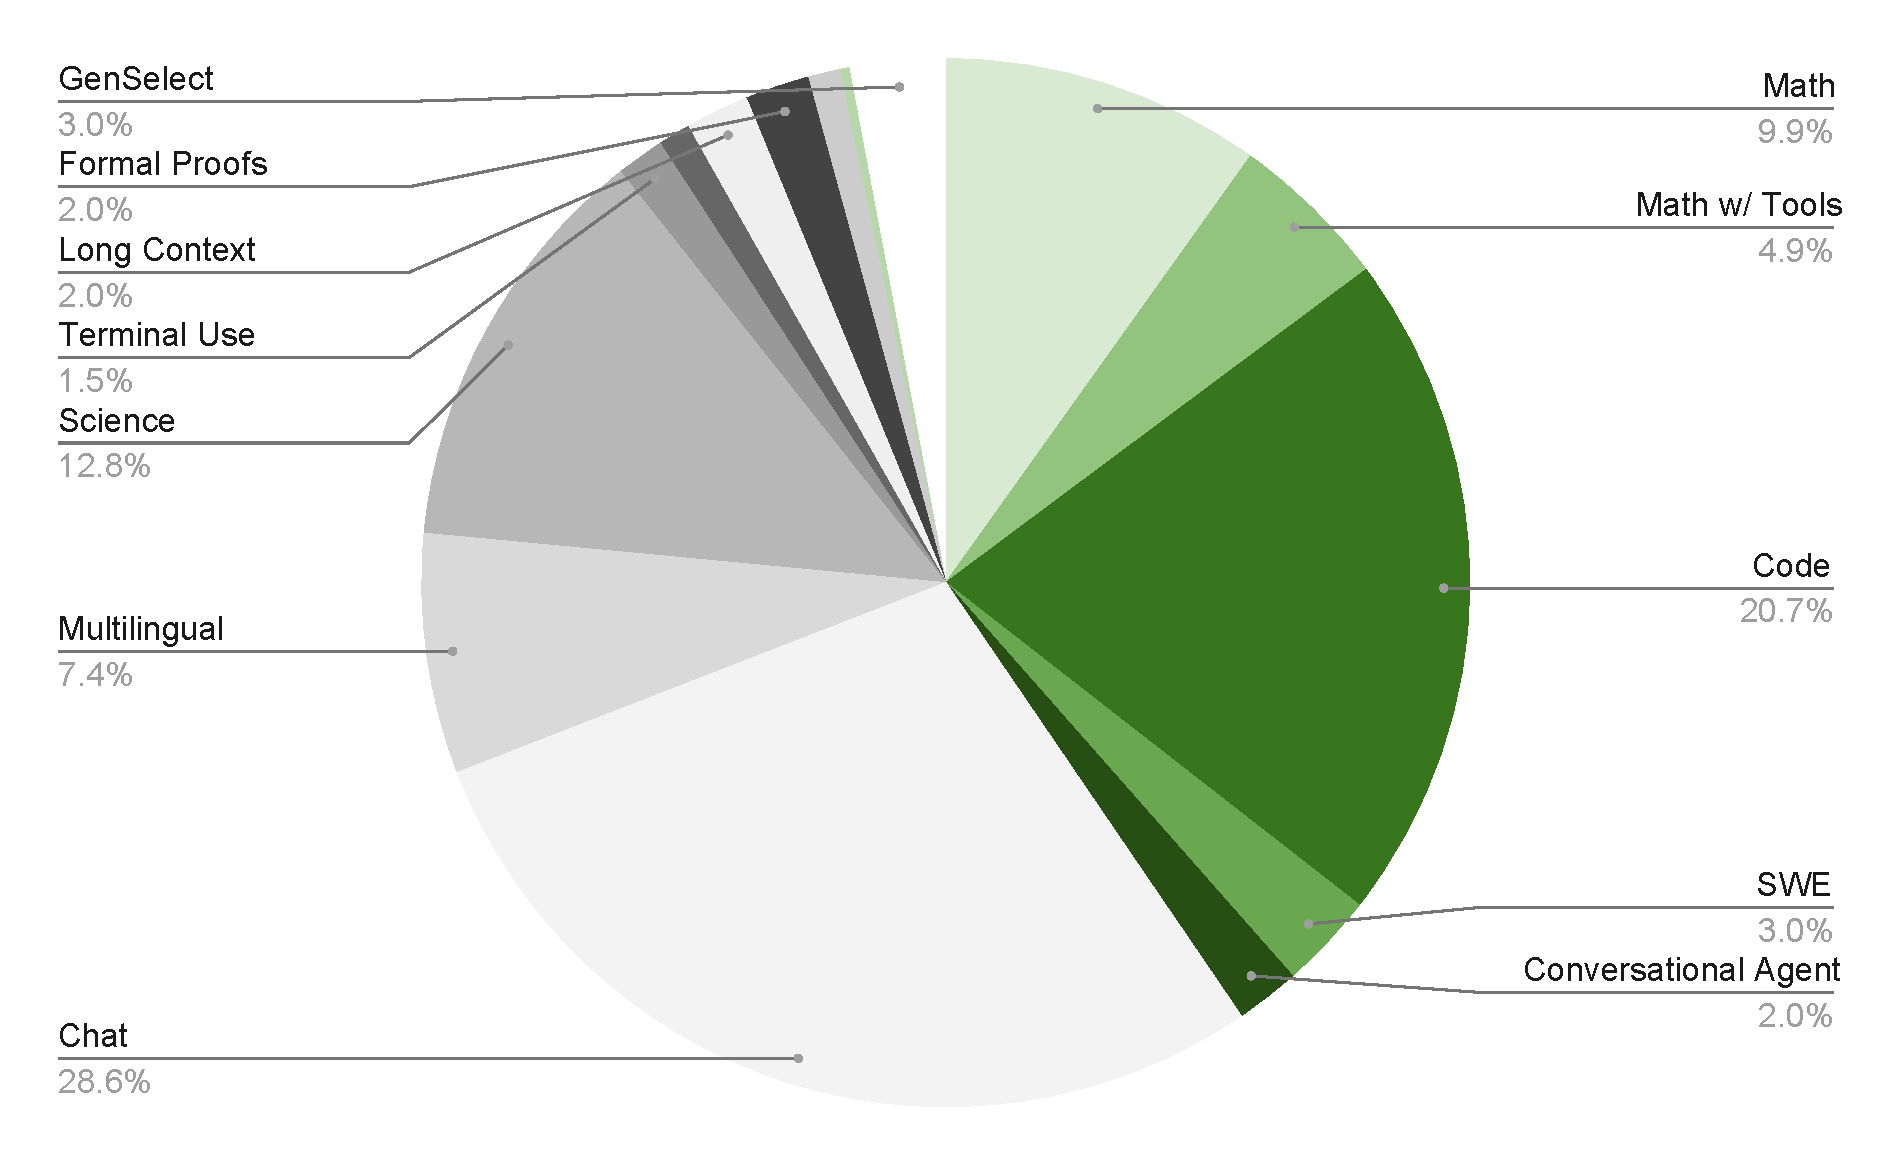
\includegraphics[width=10cm]{figures/sft_blend.pdf}
    \caption{SFT data blend for \ourmodel. }
    \label{fig:sft_blend}
\end{figure}

\subsubsection{Reasoning Control}
\ourmodel allows for two different forms of reasoning control: reasoning on/off control and token budget control. Similar to \citet{nemotronnanov2}, to enable reasoning on/off control we strip the reasoning traces from a random 10\% of samples, and to enable budget control, we randomly truncate 3\% of reasoning traces to different reasoning budgets, before continuing with the original post-reasoning response.

\subsubsection{Hyperparameters}
We train for 13000 steps using a batch size of 64 and employ sequence packing to a sequence length of 256K. We use a learning rate of $5\cdot 10^{-5}$ and use 800 steps of learning rate warmup. We use a sequence-level MoE load balancing regularizer and set the loss coefficient to $10^{-4}$.

% \todo{Soumye: Review expand}


% \subsection{Multi environment Reinforcement Learning from Verifiable Rewards}
\label{subsec:RLVR}
We employ a unified RLVR stage, training on all environments simultaneously. We find that this results in stable gains across all benchmarks throughout training, while single environment training often results in un-recoverable degradation of other benchmarks. We do two stages of such RLVR: one immediately after SFT and one after RLHF.
\subsubsection{Environments}

% \todo{Soumye. Highly suggest we give some numbers regarding the scale of each of the envs, e.g. if it is the competitive coding, how many samples with how many unit test in total? Additionally, if you want to sell the scale, we can talk about in total how many samples have been used through the RLVR stage (this could even be before we talk about details about each envs).}

\textbf{Competition Math.} We train on the DAPO \citep{yu2025dapo} and SkyWorks math \citep{he2025skywork} datasets. These datasets have 17K and 104K tasks respectively.

\textbf{Competition Coding.} We use competitive coding problems from \citet{ahmad2025opencodereasoning}. We limit the number of unit tests to 50 in order to reduce verification time. This filtering leaves us with 22K tasks.

\textbf{Question Answering.} We train on a variety of difficult multiple choice datasets focusing on STEM domains. Here the questions and answers are generated based on information from reference documents. This dataset has with 135K tasks.

\textbf{Structured Outputs.} We train \ourmodel to have strong JSON schema adherence capabilities. We utilized NeMo Data Designer \citep{nemo-data-designer} to create the seed dataset for RL. We start by constructing (JSON schema, document) pairs conditioned on diverse topics using Qwen3-235B-A22B-Instruct-2507 \citep{yang2025qwen3technicalreport}. We then utilized these pairs to create RL prompts by taking the model to summarize the document according to the schema.  To ensure high syntactic validity, the pipeline enforced strict complexity controls and applied rejection sampling, while simultaneously varying instruction difficulty and phrasing to maximize input diversity. This pipeline produces 9K tasks.

In the RL stage, a positive reward is given when the output matches the exact schema constraints, and no reward is given otherwise. For simplicity, we do not add a reward for the semantic content of the output.

\textbf{Instruction Following.} We use two instruction following environments during the training. The first environment is similar to the IFEval style environment used in \citet{bercovich2025llamanemotronefficientreasoningmodels}, but with refreshed constraints from the IFBench training set \citep{pyatkin2025generalizing}. We create 46K tasks for this environment.

The second environment uses LLM as a judge to verify whether or not the agent has followed complex instructions in multi-turn settings, where the instructions may be quite subtle. This environment is inspired by the Multi-Challenge benchmark \citep{deshpande2025multichallenge}. We create 3K total tasks for it.

\textbf{Long Context.}
We generate challenging long-context QA pairs using Qwen3-235B-A22B-Thinking-2507 \citep{yang2025qwen3technicalreport}, drawing from a subset of our pre-training mixture designed for multi-document synthesis. Each question is required to reference at least five documents, with the total input limited to 32k tokens. We employ Qwen3-235B-A22B-Instruct-2507 \citep{yang2025qwen3technicalreport} as the LLM judge to evaluate the model's rollouts. This dataset contains 12K tasks.

\textbf{Agentic Tool Use.} We use two environments to improve tool use capabilities. The first is Workplace Assistant, a multi-step verifiable tool-calling setup adapted from Styles \citep{Styles2024WorkBench} that was also used in Nemotron 2 Nano \citep{nemotronnanov2}. This is a tool use - multi step agentic environment that tests the agent's ability to execute tasks in a workplace setting. Workplace Assistant contains a sandbox environment with five databases, 26 tools, and 690 tasks. These tasks represent common business activities, such as sending emails, scheduling meetings, etc. The correctness is verified through executing the tool calls issued by the agent and comparing it to the ground truth database state. 

The second environment is a Multi-turn conversational agent environment. It tests an agent's tool-calling and proactive asking capability. Comprising approximately 1K tasks, this environment simulates complex banking scenarios like assisting customers with unblocking a credit card or solving account disputes. The correctness of the agent's actions is automatically verified by executing the tool calls it issues and comparing the resulting database state against the predefined ground truth.



\subsubsection{Data Mixture and Curriculum}
We begin by profiling all reinforcement learning (RL) tasks using our supervised fine-tuning (SFT) checkpoint. To focus training on challenging cases, we filter out samples where the SFT checkpoint already achieves a 100\% pass rate. We then adopt the curriculum training method introduced in~\citet{bercovich2025llamanemotronefficientreasoningmodels}, which dynamically adjusts task difficulty throughout training.

In each batch, we maintain a fixed ratio of samples across different domains. For each domain, we model the target pass-rate distribution as a Gaussian function, shifting from high pass-rate (easier) samples early in training to low pass-rate (harder) samples later. The target mean of Gaussian distribution decreases linearly throughout training steps. Within each batch, samples from different domains are shuffled. This Gaussian sampling strategy prevents overfitting to either overly easy or overly difficult examples, ensuring a balanced learning progression. 

This approach enables a controlled and gradual increase in task difficulty while preserving domain diversity and ensuring efficient batch composition. Figure~\ref{fig:pass_rate} illustrates how sample difficulty evolves over the course of RL training. Once training progress plateaus, we re-profile the tasks using the best RL checkpoint and construct a new curriculum to further refine performance.

\begin{figure}[ht]
    \centering
    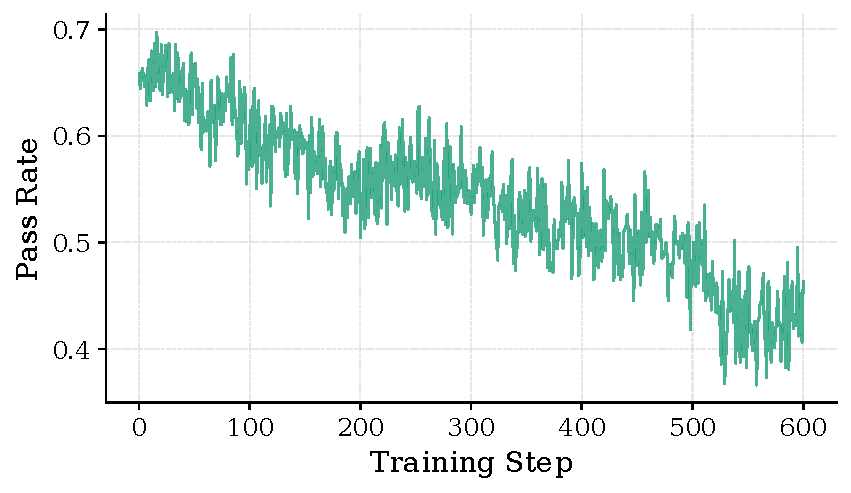
\includegraphics[width=0.6\textwidth]{figures/pass_rate.pdf}
    \caption{Batch-wise pass rates across the RL curriculum.}
    \label{fig:pass_rate}
\end{figure}

We compare curriculum sampling against random sampling using an intermediate SFT checkpoint, maintaining identical domain ratios in both cases. As shown in Figure~\ref{fig:curriculum_ablation}, curriculum sampling ensures stable learning across multiple domains throughout training. In contrast, random sampling biases the model toward easier tasks, preventing it from effectively learning more challenging ones.

\begin{figure}[ht]
    \centering
    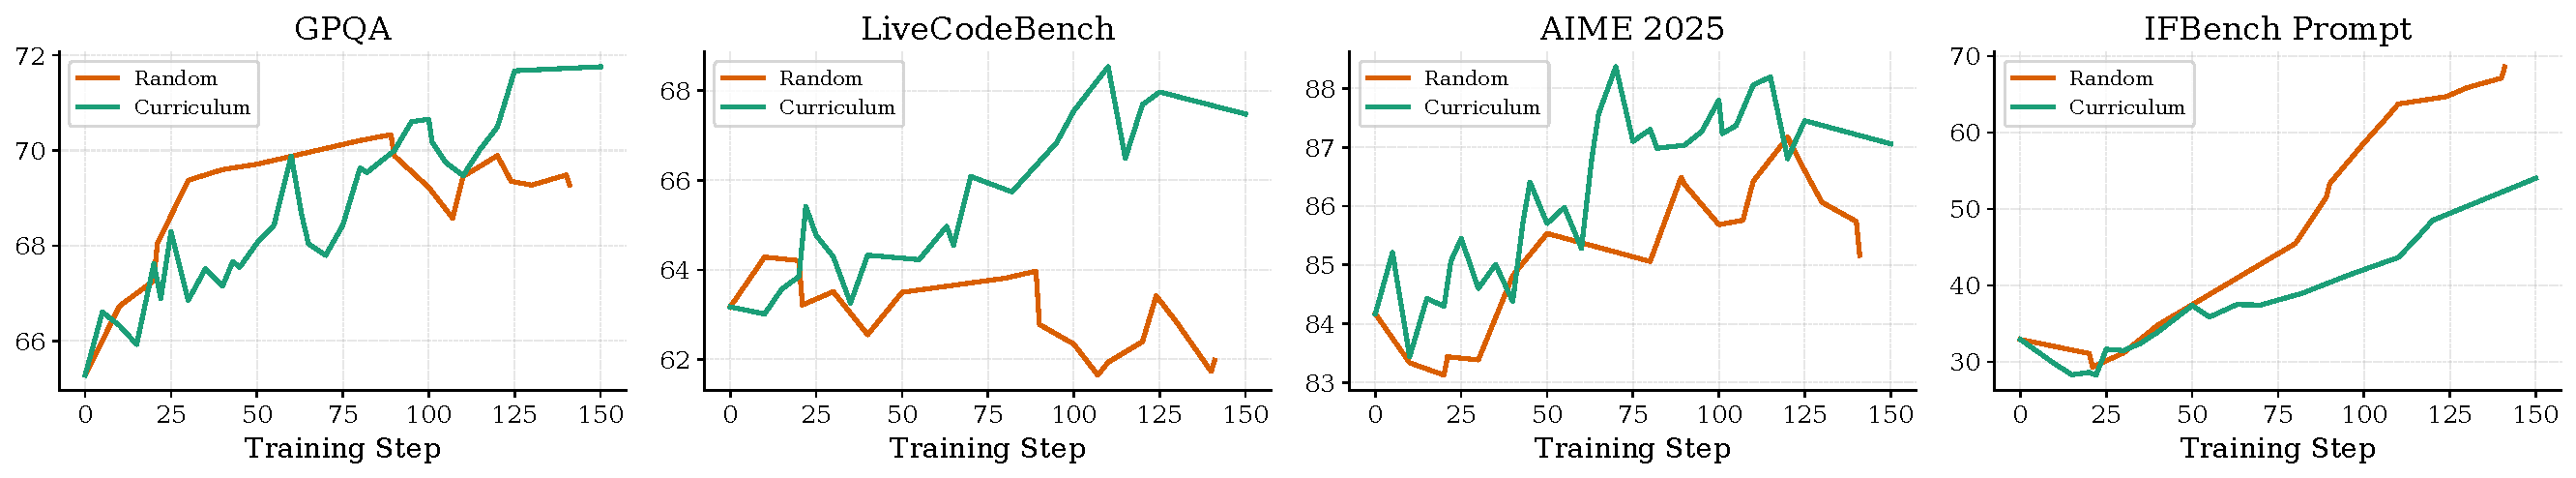
\includegraphics[width=\textwidth]{figures/rlvr_compare_curriculum.pdf}
    \caption{Comparison between curriculum sampling and random sampling.}
    \label{fig:curriculum_ablation}
\end{figure}

\subsubsection{Surpassing SFT with RLVR}

Recent works have demonstrated that supervised fine-tuning (SFT) alone on small models can achieve strong performance~\citep{ahmad2025opencodereasoning,deepseekai2025deepseekr1incentivizingreasoningcapability}. In this study, we investigate whether RLVR can outperform a heavily fine-tuned SFT baseline. As illustrated in Figure~\ref{fig:surpass_sft_with_rlvr}, we compare the accuracy of model during RLVR training with two SFT checkpoints: 
\begin{itemize} 
\item SFT1: Our initial RLVR starting point, fine-tuned for approximately 3 epochs. 
\item SFT2: A heavily fine-tuned checkpoint, trained to full convergence (approximately 5 epochs). \end{itemize} 
Our results show that even with relatively short training, RLVR consistently exceeds  or matches the accuracy of the heavily fine-tuned SFT model across all evaluated domains.
\begin{figure}[ht]
    \centering
    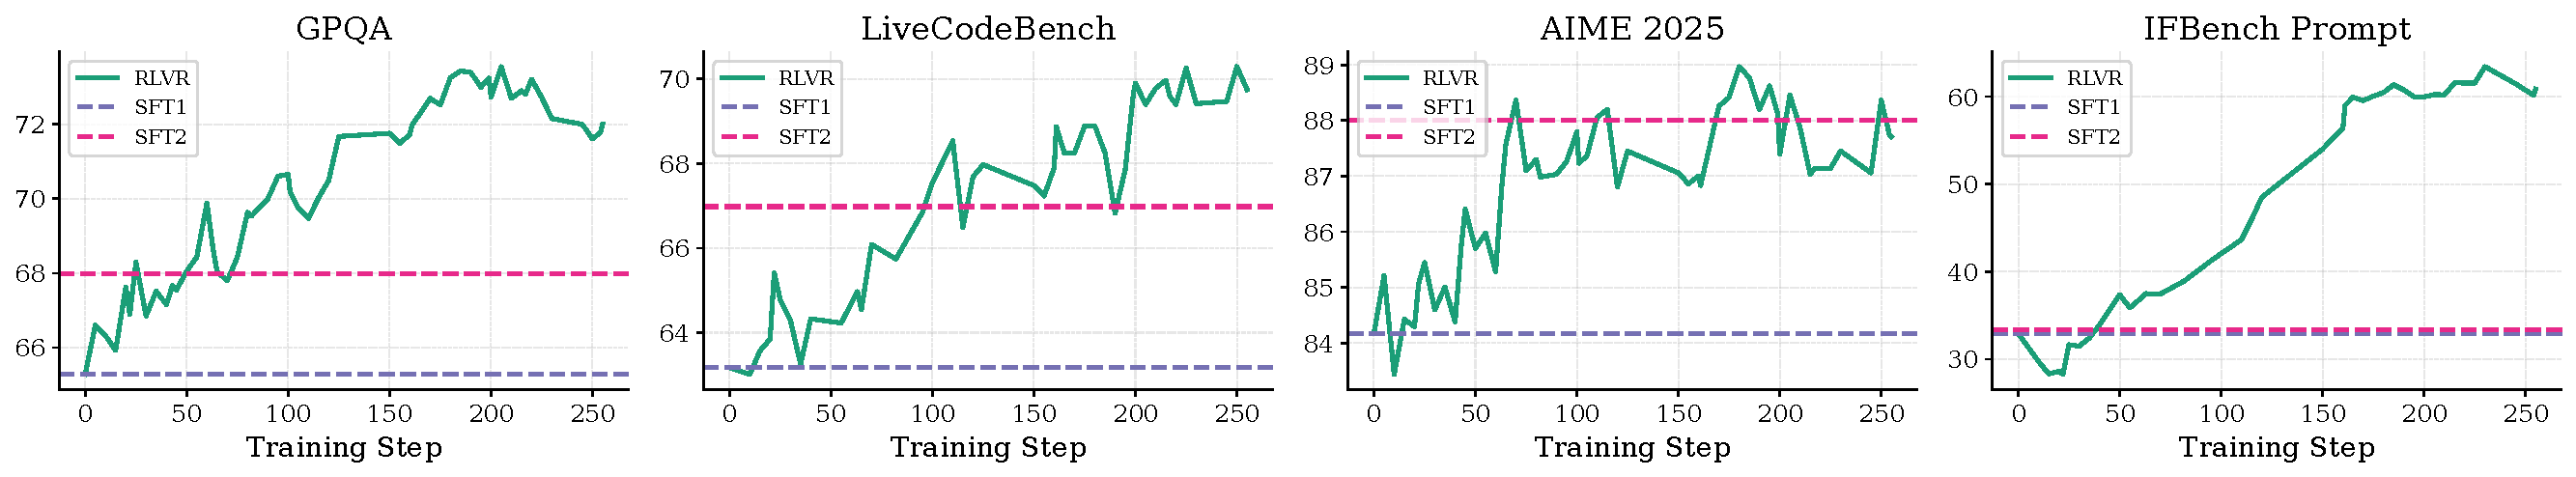
\includegraphics[width=\textwidth]{figures/rlvr_surpass_sft.pdf}
    \caption{RLVR surpasses or matches heavily fine-tuned SFT model across all evaluated domains.}
    \label{fig:surpass_sft_with_rlvr}
\end{figure}


\subsubsection{Infrastructure}
\label{subsubsection:RLinfra}

RL at the frontier of model post-training is currently defined by scaling up to an increasing diversity of tasks or environments designed for the model to learn increasingly general capabilities.
Scaling RL to many environments requires a high-performance, extensible, and standardized interface for coordinating between rollouts and training.
To address the scaling performance and extensibility challenges using one standard framework, we adopt NeMo Gym \citep{nemo-gym} and NeMo RL \citep{nemo-rl} for enabling large-scale RL on many different environments/verifiers.

NeMo Gym is based on the abstraction of \emph{servers}.
There are three core varieties of servers in Gym: (1) \emph{agents}, (2) \emph{models}, and (3) \emph{resources}.
An \emph{agent} server implements the rollout kernel of a RL environment.
A \emph{model} server wraps an inference engine such as vLLM \citep{kwon2023efficientmemorymanagementlarge} to provide a prompt-response API, and also carefully preserves token and inference log-prob data and metadata required for RL.
A \emph{resource} server provides a verification API for computing rewards from a given rollout.

Our Nemotron Nano 3 RLVR experiments were all based on an integrated infrastructure of NeMo RL and NeMo Gym:
NeMo RL acts as the RL training loop controller, using Megatron-Core \citep{shoeybi2020megatronlmtrainingmultibillionparameter} for model training at scale, and routing all rollouts through NeMo Gym and vLLM.

\subsubsection{Algorithm}
\label{sec:rl-algo}
We train \ourmodel using synchronous GRPO with masked importance sampling to mitigate training-inference misalignment \citep{Shao2024DeepSeekMath, team2025every, yao2025offpolicy}. We use 128 prompts per step and use 16 generations per prompt. We train with a batch size of 2048, making our updates on-policy. To further stabilize training we also freeze the MoE router weights. We employ the aux-loss-free load balancing approach and keep updating expert bias~\citep{wang2024auxiliary}. 

Our entire training run is done with a maximum generation length of 49K. We use overlong filtering \citep{yu2025dapo}, which we find boosts performance on reasoning intensive benchmarks.


% \subsubsection{SFT Initialization}
% \todo{Peter, Alex?: Early, medium, late SFT ckpt}


\begin{figure}[ht]
    \centering
    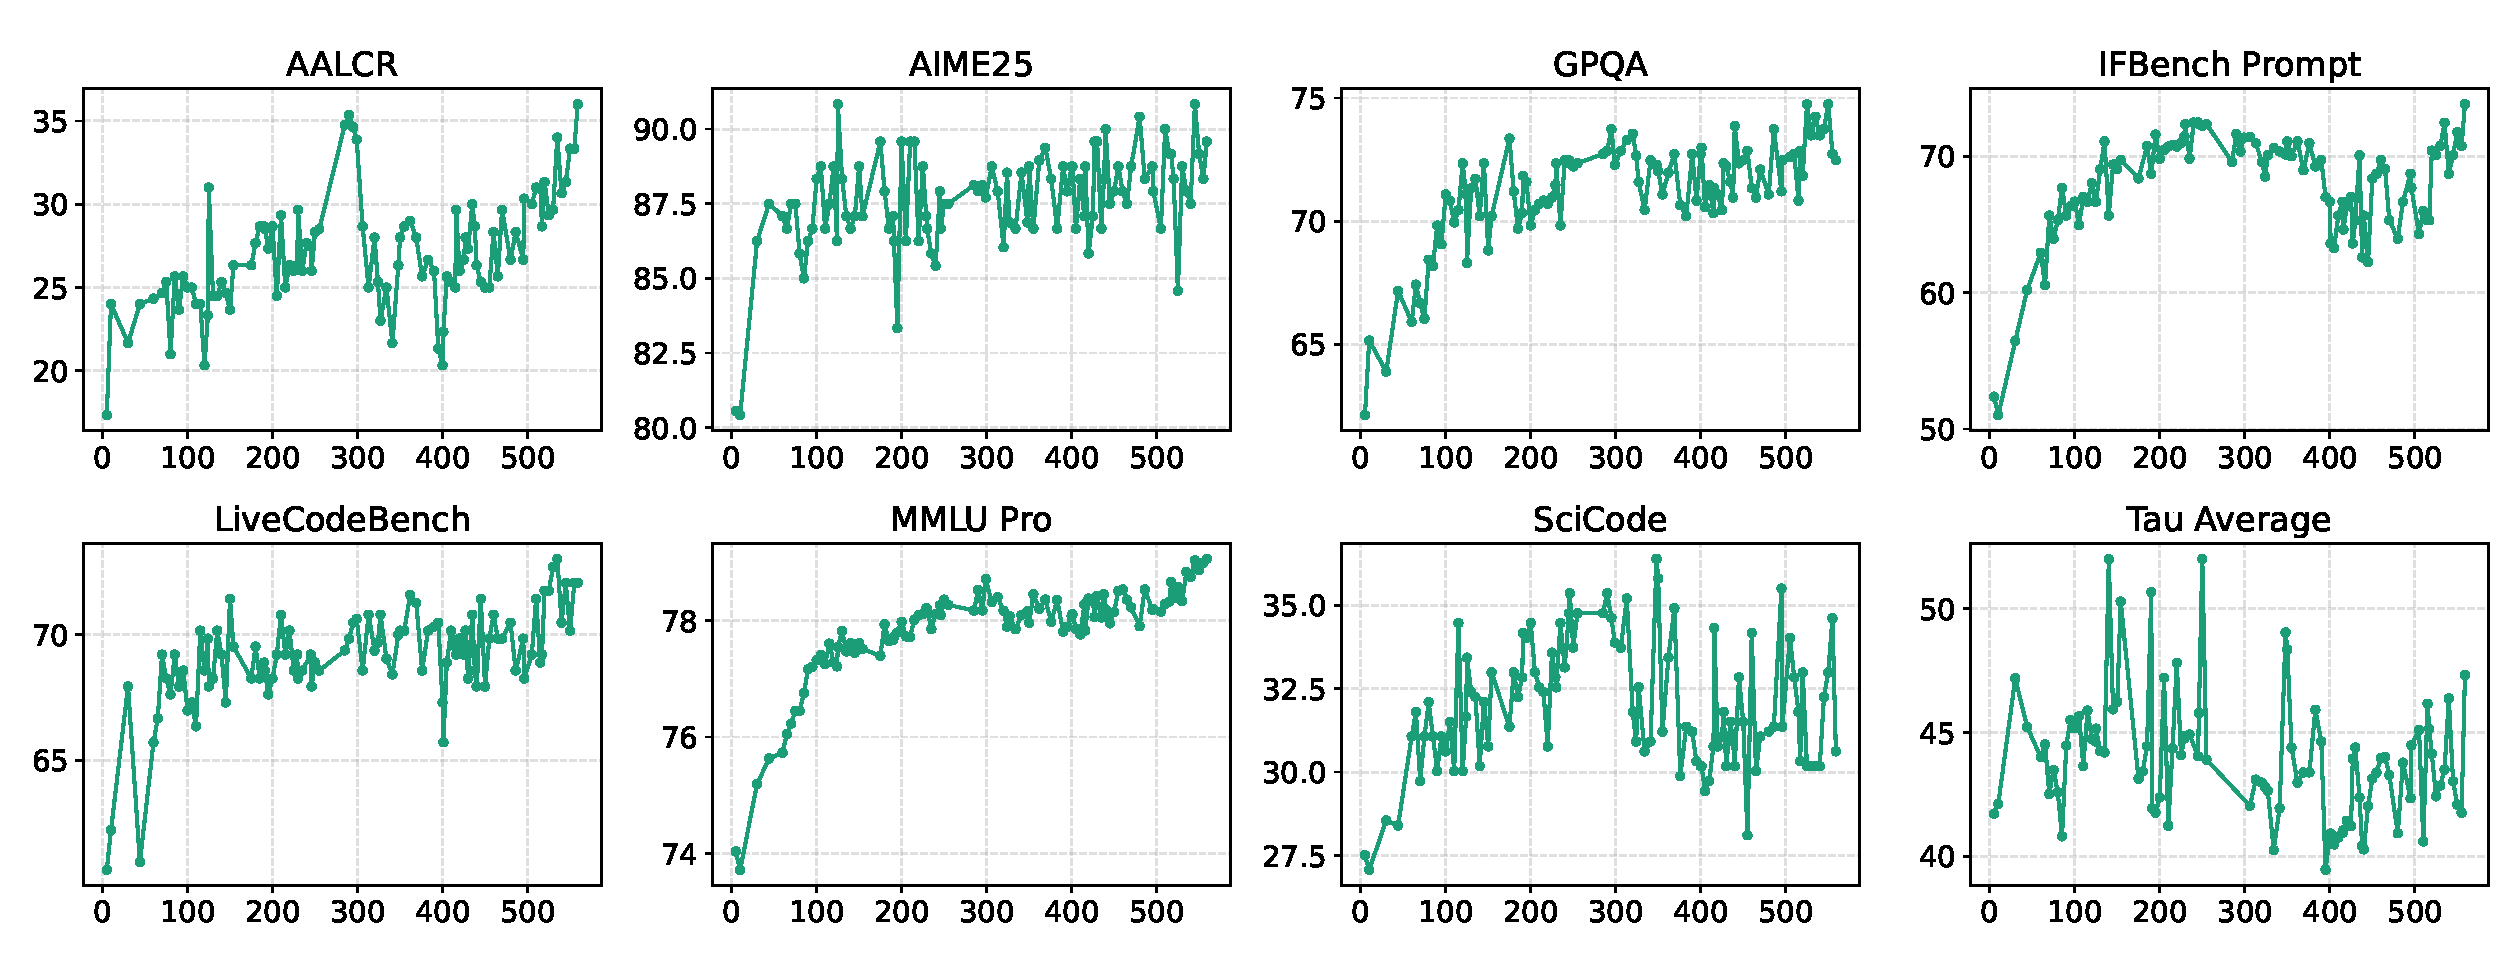
\includegraphics[width=\textwidth]{figures/rl_progress_concat.pdf}
    \caption{Benchmark performance throughout RL training.}
    \label{fig:rl_progress}
\end{figure}
\subsection{Multi environment Reinforcement Learning from Verifiable Rewards}
\label{subsec:RLVR}
We employ a unified RLVR stage, training on all environments simultaneously. We find that this results in stable gains across all benchmarks throughout training, while single environment training often results in un-recoverable degradation of other benchmarks. We do two stages of such RLVR: one immediately after SFT and one after RLHF.
\subsubsection{Environments}

% \todo{Soumye. Highly suggest we give some numbers regarding the scale of each of the envs, e.g. if it is the competitive coding, how many samples with how many unit test in total? Additionally, if you want to sell the scale, we can talk about in total how many samples have been used through the RLVR stage (this could even be before we talk about details about each envs).}

\textbf{Competition Math.} We train on the DAPO \citep{yu2025dapo} and SkyWorks math \citep{he2025skywork} datasets. These datasets have 17K and 104K tasks respectively.

\textbf{Competition Coding.} We use competitive coding problems from \citet{ahmad2025opencodereasoning}. We limit the number of unit tests to 50 in order to reduce verification time. This filtering leaves us with 22K tasks.

\textbf{Question Answering.} We train on a variety of difficult multiple choice datasets focusing on STEM domains. Here the questions and answers are generated based on information from reference documents. This dataset has with 135K tasks.

\textbf{Structured Outputs.} We train \ourmodel to have strong JSON schema adherence capabilities. We utilized NeMo Data Designer \citep{nemo-data-designer} to create the seed dataset for RL. We start by constructing (JSON schema, document) pairs conditioned on diverse topics using Qwen3-235B-A22B-Instruct-2507 \citep{yang2025qwen3technicalreport}. We then utilized these pairs to create RL prompts by taking the model to summarize the document according to the schema.  To ensure high syntactic validity, the pipeline enforced strict complexity controls and applied rejection sampling, while simultaneously varying instruction difficulty and phrasing to maximize input diversity. This pipeline produces 9K tasks.

In the RL stage, a positive reward is given when the output matches the exact schema constraints, and no reward is given otherwise. For simplicity, we do not add a reward for the semantic content of the output.

\textbf{Instruction Following.} We use two instruction following environments during the training. The first environment is similar to the IFEval style environment used in \citet{bercovich2025llamanemotronefficientreasoningmodels}, but with refreshed constraints from the IFBench training set \citep{pyatkin2025generalizing}. We create 46K tasks for this environment.

The second environment uses LLM as a judge to verify whether or not the agent has followed complex instructions in multi-turn settings, where the instructions may be quite subtle. This environment is inspired by the Multi-Challenge benchmark \citep{deshpande2025multichallenge}. We create 3K total tasks for it.

\textbf{Long Context.}
We generate challenging long-context QA pairs using Qwen3-235B-A22B-Thinking-2507 \citep{yang2025qwen3technicalreport}, drawing from a subset of our pre-training mixture designed for multi-document synthesis. Each question is required to reference at least five documents, with the total input limited to 32k tokens. We employ Qwen3-235B-A22B-Instruct-2507 \citep{yang2025qwen3technicalreport} as the LLM judge to evaluate the model's rollouts. This dataset contains 12K tasks.

\textbf{Agentic Tool Use.} We use two environments to improve tool use capabilities. The first is Workplace Assistant, a multi-step verifiable tool-calling setup adapted from Styles \citep{Styles2024WorkBench} that was also used in Nemotron 2 Nano \citep{nemotronnanov2}. This is a tool use - multi step agentic environment that tests the agent's ability to execute tasks in a workplace setting. Workplace Assistant contains a sandbox environment with five databases, 26 tools, and 690 tasks. These tasks represent common business activities, such as sending emails, scheduling meetings, etc. The correctness is verified through executing the tool calls issued by the agent and comparing it to the ground truth database state. 

The second environment is a Multi-turn conversational agent environment. It tests an agent's tool-calling and proactive asking capability. Comprising approximately 1K tasks, this environment simulates complex banking scenarios like assisting customers with unblocking a credit card or solving account disputes. The correctness of the agent's actions is automatically verified by executing the tool calls it issues and comparing the resulting database state against the predefined ground truth.



\subsubsection{Data Mixture and Curriculum}
We begin by profiling all reinforcement learning (RL) tasks using our supervised fine-tuning (SFT) checkpoint. To focus training on challenging cases, we filter out samples where the SFT checkpoint already achieves a 100\% pass rate. We then adopt the curriculum training method introduced in~\citet{bercovich2025llamanemotronefficientreasoningmodels}, which dynamically adjusts task difficulty throughout training.

In each batch, we maintain a fixed ratio of samples across different domains. For each domain, we model the target pass-rate distribution as a Gaussian function, shifting from high pass-rate (easier) samples early in training to low pass-rate (harder) samples later. The target mean of Gaussian distribution decreases linearly throughout training steps. Within each batch, samples from different domains are shuffled. This Gaussian sampling strategy prevents overfitting to either overly easy or overly difficult examples, ensuring a balanced learning progression. 

This approach enables a controlled and gradual increase in task difficulty while preserving domain diversity and ensuring efficient batch composition. Figure~\ref{fig:pass_rate} illustrates how sample difficulty evolves over the course of RL training. Once training progress plateaus, we re-profile the tasks using the best RL checkpoint and construct a new curriculum to further refine performance.

\begin{figure}[ht]
    \centering
    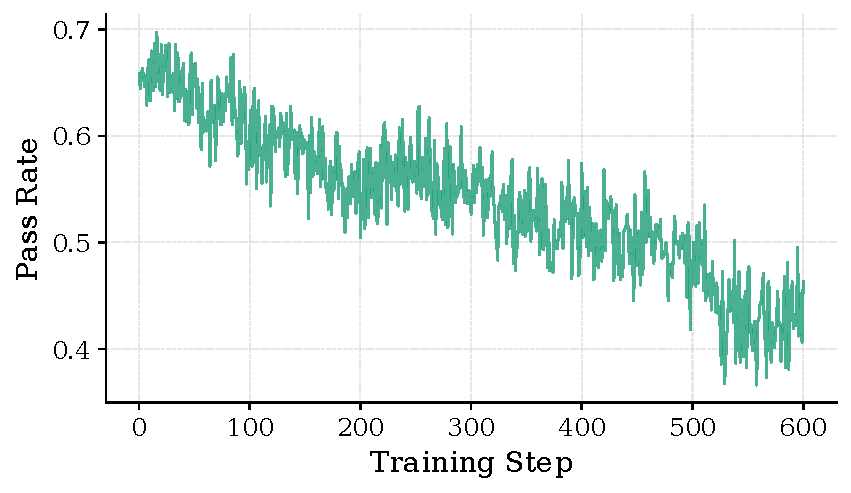
\includegraphics[width=0.6\textwidth]{figures/pass_rate.pdf}
    \caption{Batch-wise pass rates across the RL curriculum.}
    \label{fig:pass_rate}
\end{figure}

We compare curriculum sampling against random sampling using an intermediate SFT checkpoint, maintaining identical domain ratios in both cases. As shown in Figure~\ref{fig:curriculum_ablation}, curriculum sampling ensures stable learning across multiple domains throughout training. In contrast, random sampling biases the model toward easier tasks, preventing it from effectively learning more challenging ones.

\begin{figure}[ht]
    \centering
    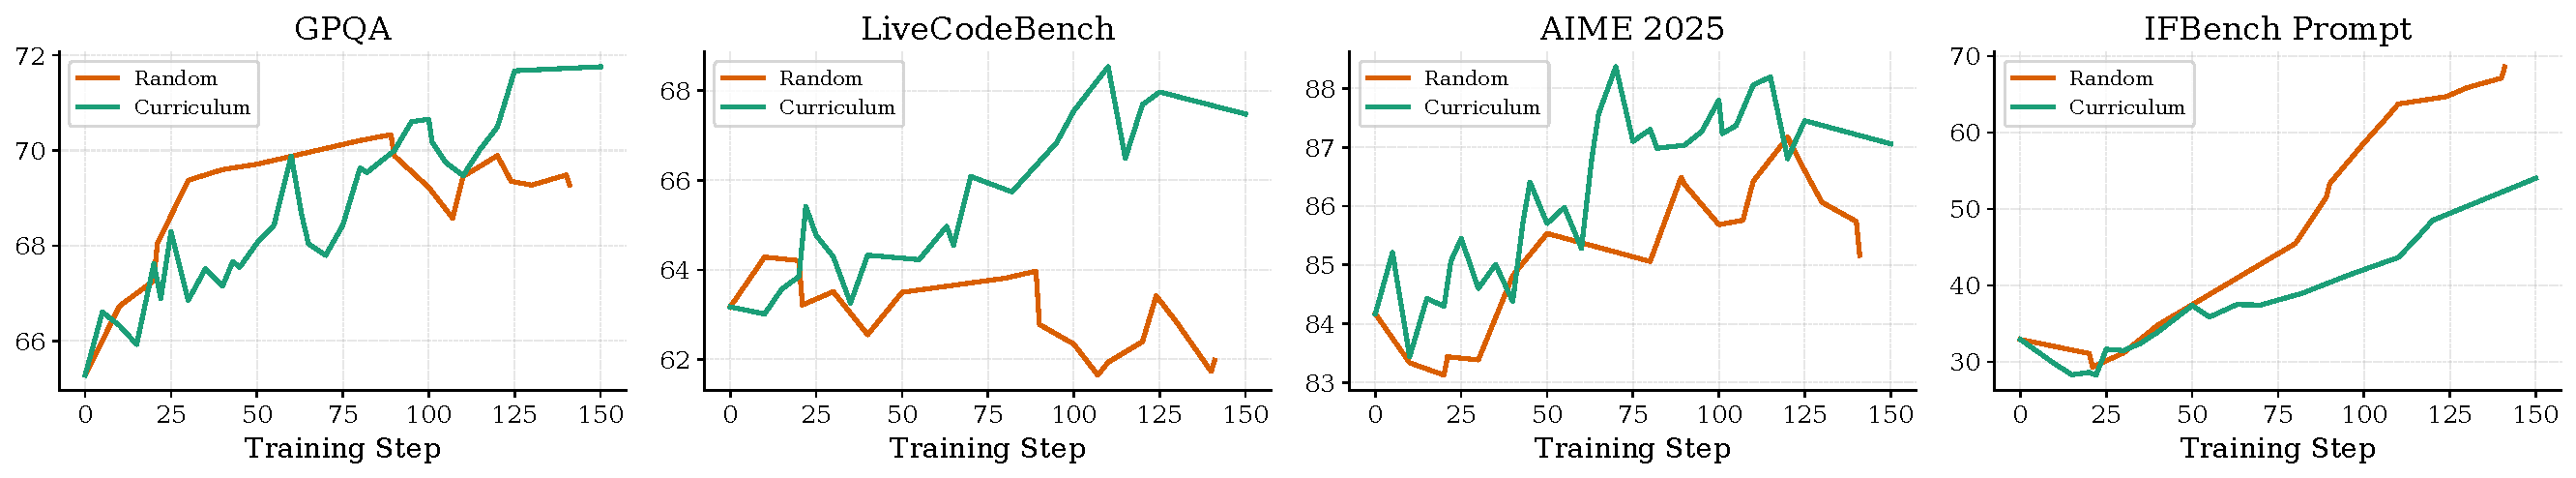
\includegraphics[width=\textwidth]{figures/rlvr_compare_curriculum.pdf}
    \caption{Comparison between curriculum sampling and random sampling.}
    \label{fig:curriculum_ablation}
\end{figure}

\subsubsection{Surpassing SFT with RLVR}

Recent works have demonstrated that supervised fine-tuning (SFT) alone on small models can achieve strong performance~\citep{ahmad2025opencodereasoning,deepseekai2025deepseekr1incentivizingreasoningcapability}. In this study, we investigate whether RLVR can outperform a heavily fine-tuned SFT baseline. As illustrated in Figure~\ref{fig:surpass_sft_with_rlvr}, we compare the accuracy of model during RLVR training with two SFT checkpoints: 
\begin{itemize} 
\item SFT1: Our initial RLVR starting point, fine-tuned for approximately 3 epochs. 
\item SFT2: A heavily fine-tuned checkpoint, trained to full convergence (approximately 5 epochs). \end{itemize} 
Our results show that even with relatively short training, RLVR consistently exceeds  or matches the accuracy of the heavily fine-tuned SFT model across all evaluated domains.
\begin{figure}[ht]
    \centering
    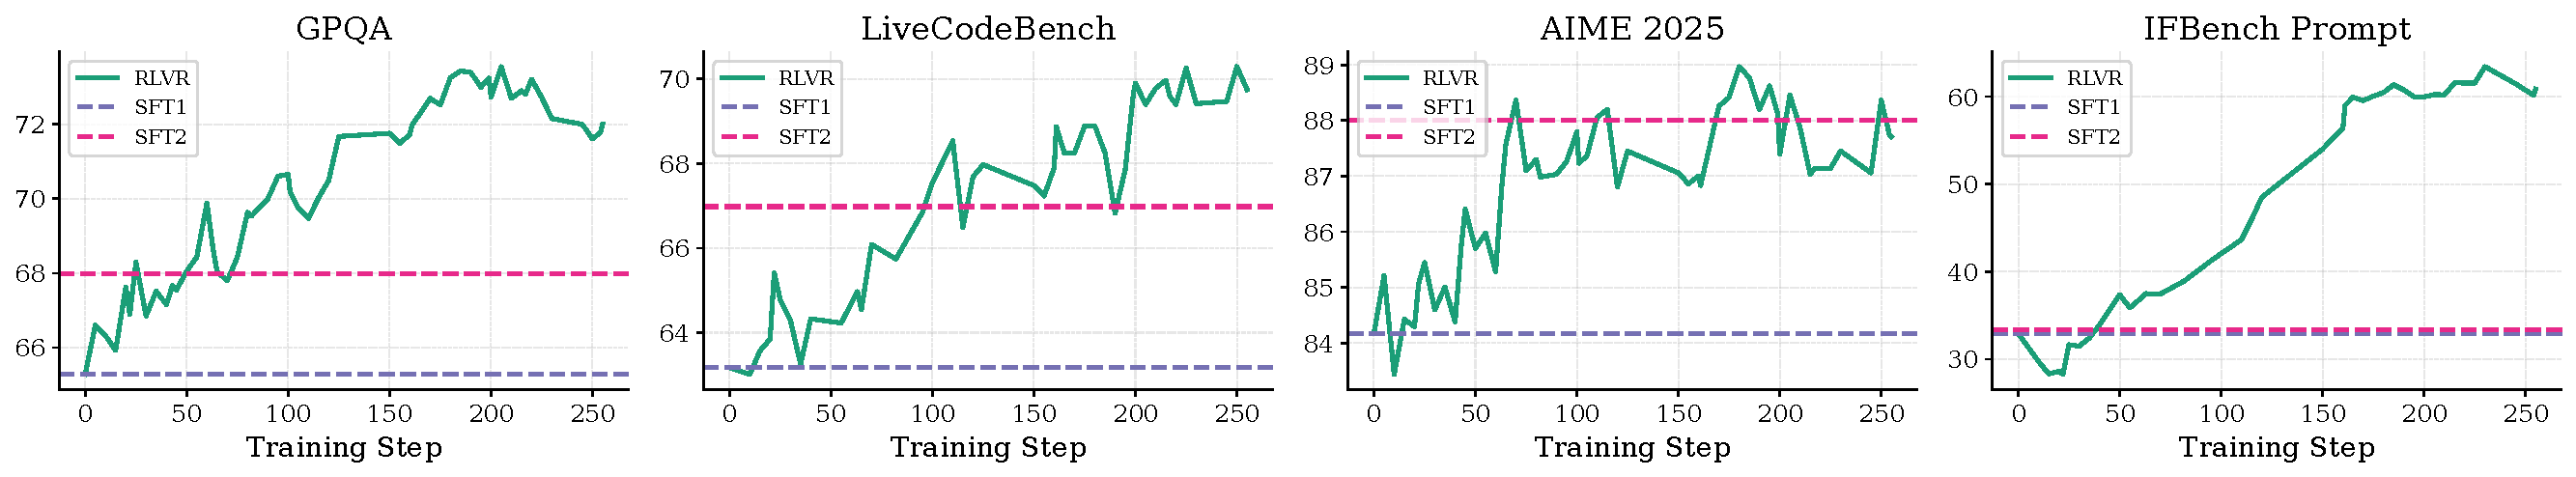
\includegraphics[width=\textwidth]{figures/rlvr_surpass_sft.pdf}
    \caption{RLVR surpasses or matches heavily fine-tuned SFT model across all evaluated domains.}
    \label{fig:surpass_sft_with_rlvr}
\end{figure}


\subsubsection{Infrastructure}
\label{subsubsection:RLinfra}

RL at the frontier of model post-training is currently defined by scaling up to an increasing diversity of tasks or environments designed for the model to learn increasingly general capabilities.
Scaling RL to many environments requires a high-performance, extensible, and standardized interface for coordinating between rollouts and training.
To address the scaling performance and extensibility challenges using one standard framework, we adopt NeMo Gym \citep{nemo-gym} and NeMo RL \citep{nemo-rl} for enabling large-scale RL on many different environments/verifiers.

NeMo Gym is based on the abstraction of \emph{servers}.
There are three core varieties of servers in Gym: (1) \emph{agents}, (2) \emph{models}, and (3) \emph{resources}.
An \emph{agent} server implements the rollout kernel of a RL environment.
A \emph{model} server wraps an inference engine such as vLLM \citep{kwon2023efficientmemorymanagementlarge} to provide a prompt-response API, and also carefully preserves token and inference log-prob data and metadata required for RL.
A \emph{resource} server provides a verification API for computing rewards from a given rollout.

Our Nemotron Nano 3 RLVR experiments were all based on an integrated infrastructure of NeMo RL and NeMo Gym:
NeMo RL acts as the RL training loop controller, using Megatron-Core \citep{shoeybi2020megatronlmtrainingmultibillionparameter} for model training at scale, and routing all rollouts through NeMo Gym and vLLM.

\subsubsection{Algorithm}
\label{sec:rl-algo}
We train \ourmodel using synchronous GRPO with masked importance sampling to mitigate training-inference misalignment \citep{Shao2024DeepSeekMath, team2025every, yao2025offpolicy}. We use 128 prompts per step and use 16 generations per prompt. We train with a batch size of 2048, making our updates on-policy. To further stabilize training we also freeze the MoE router weights. We employ the aux-loss-free load balancing approach and keep updating expert bias~\citep{wang2024auxiliary}. 

Our entire training run is done with a maximum generation length of 49K. We use overlong filtering \citep{yu2025dapo}, which we find boosts performance on reasoning intensive benchmarks.


% \subsubsection{SFT Initialization}
% \todo{Peter, Alex?: Early, medium, late SFT ckpt}


\begin{figure}[ht]
    \centering
    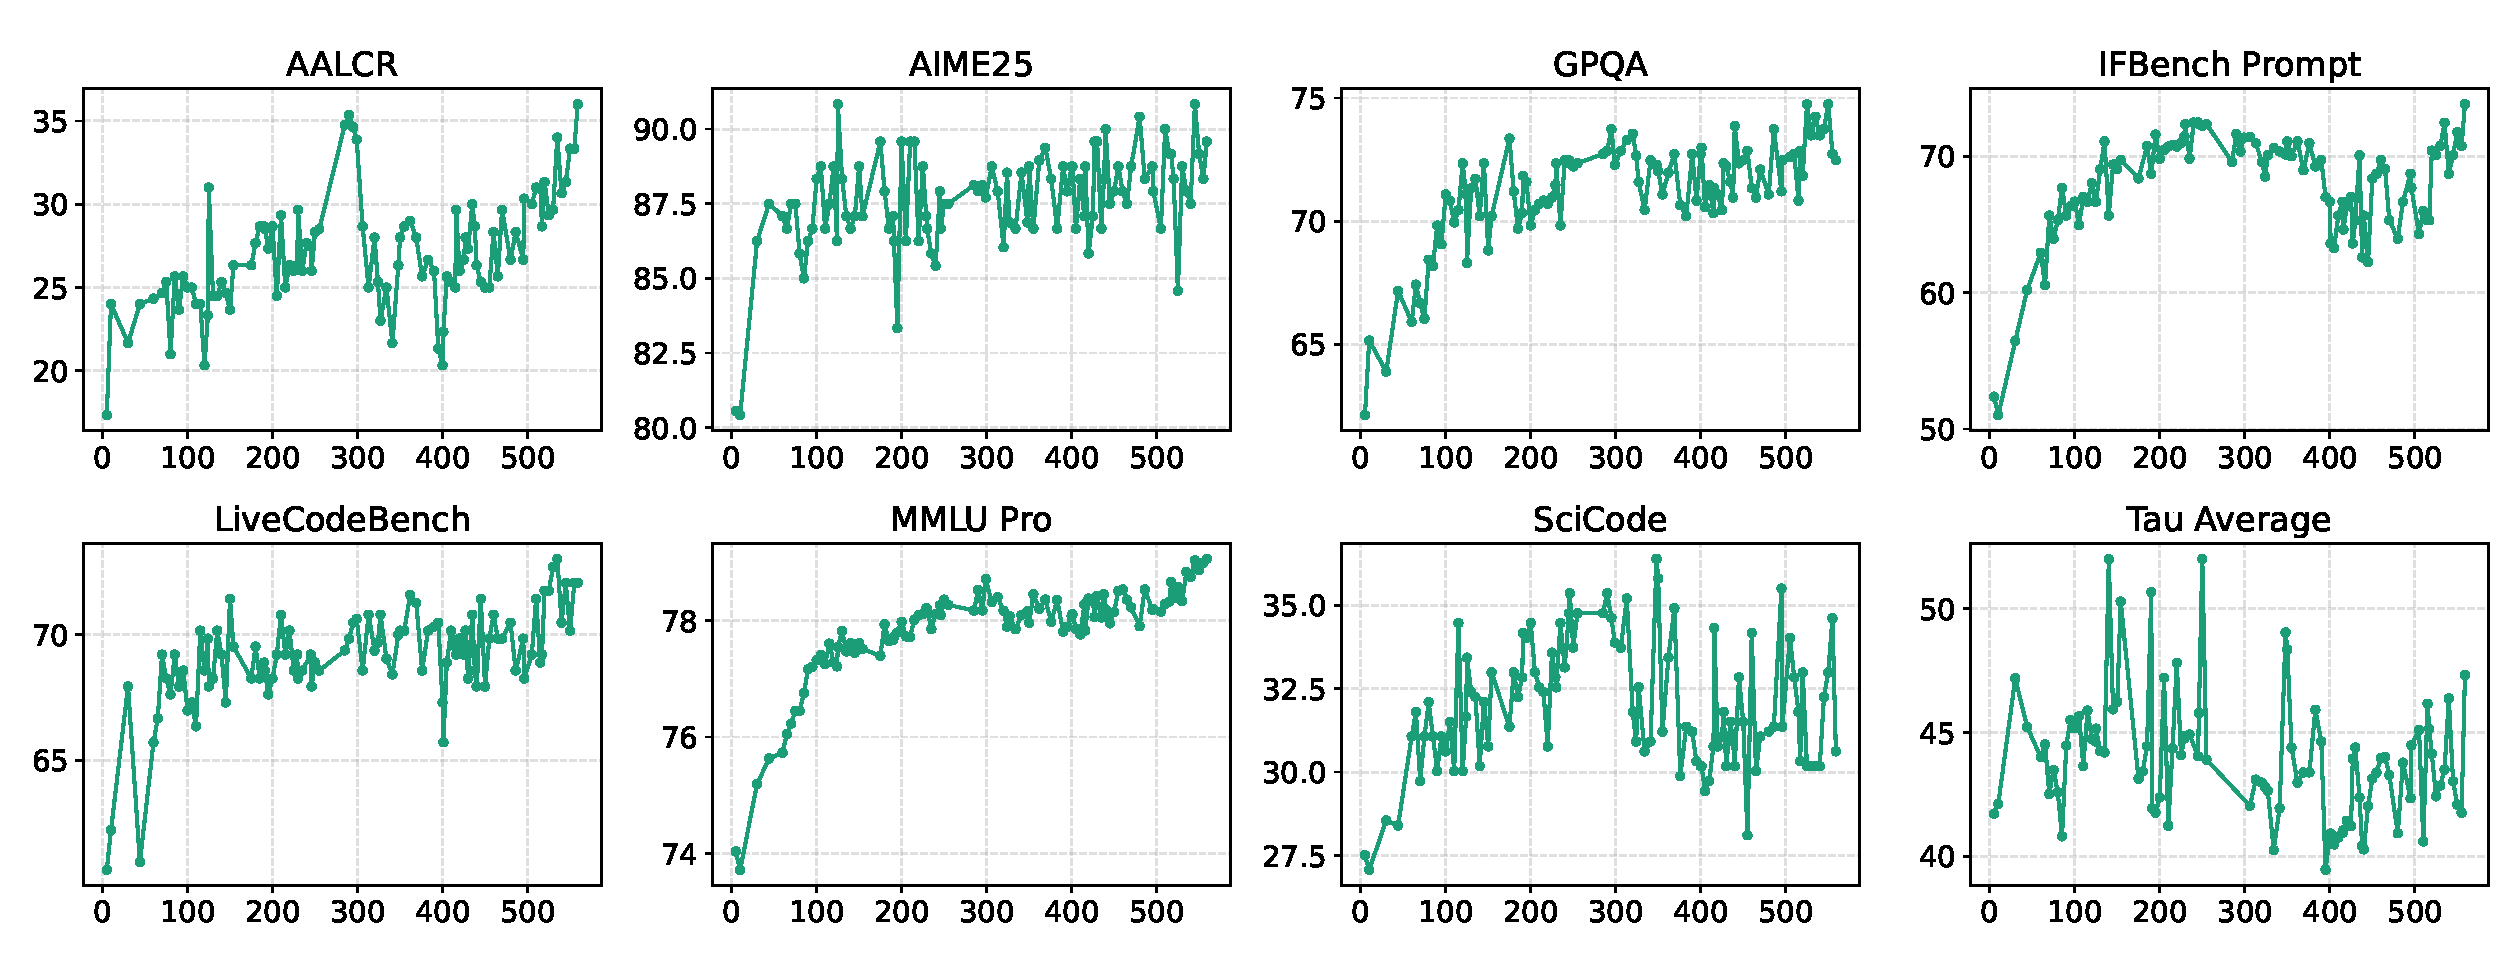
\includegraphics[width=\textwidth]{figures/rl_progress_concat.pdf}
    \caption{Benchmark performance throughout RL training.}
    \label{fig:rl_progress}
\end{figure}
\subsection{Reinforcement Learning from Human Feedback}
\label{subsec:RLHF}

\subsubsection{Scaling Reinforcement Learning for Generative Reward‑Model Training}
Many recent works \citep{deepseek-genrm,helpsteer3-pref,rmr1} have demonstrated that generative reward models (GenRMs) generalize better than traditional Bradley‑Terry models, reducing the risk of reward hacking during RLHF. In order to train an accurate and robust GenRM, we leverage reinforcement learning at scale. Building on the methodology of \citet{helpsteer3-pref}, we train Qwen3-235B-A22B-Thinking-2507~\citep{yang2025qwen3technicalreport} to become a GenRM with GRPO algorithm.  Given the conversation history, a new user request, and two candidate assistant responses, the GenRM first reasons through the strength and weakness of both responses, then produce an individual helpfulness score for each response as well as a ranking score. For GenRM training, we use 128 prompts per batch, 8 generations per prompt, and do one gradient step on the full batch. We define the reward as

\begin{align}
    \mathbf{R} = -C_1I_{\text{format}} -
    \left| P_{h1} - G_{h1} \right| - \left| P_{h2} - G_{h2} \right| - C_2 \left| P_r - G_r \right|,
\end{align}

where $P_r$, $G_r$ denote the predicted and ground-truth preference rankings; $P_{h1}$, $G_{h1}$, $P_{h2}$, $G_{h2}$ denote the predicted and ground-truth helpfulness scores for responses 1 and 2, respectively;  $I_{format}$ indicates whether the prediction violates the format requirement; $C_1$ and $C_2$ are hyper-parameters controlling the weights. We set $C_1=10$ and $C_2=1$. 

We leverage data from HelpSteer3~\citep{helpsteer3-pref}, a commercially-friendly subset of lmarena-ai/arena-human-preference-140k~\citep{chiang2024chatbot}, and a synthetic safety blend (see details in Appendix~\ref{sec:safety_pref_data}) for model training. In our dataset, individual helpfulness scores range from 1 to 5, where higher means more helpful, while ranking score ranges from 1 to 6, in which 1 denotes that response 1 is far superior to response 2 and 6 denotes that response 2 is far superior to response 1~\citep{helpsteer3-pref}. We augment each sample by switching positions of two responses to prevent positional bias. Figure~\ref{fig:genrm-training} demonstrates that the performance of GenRM on RM-Bench~\citep{rmbench}, JudgeBench~\citep{judgebench}, and our internal validation set steadily improves as training progresses.

\begin{figure}[ht]
    \centering
    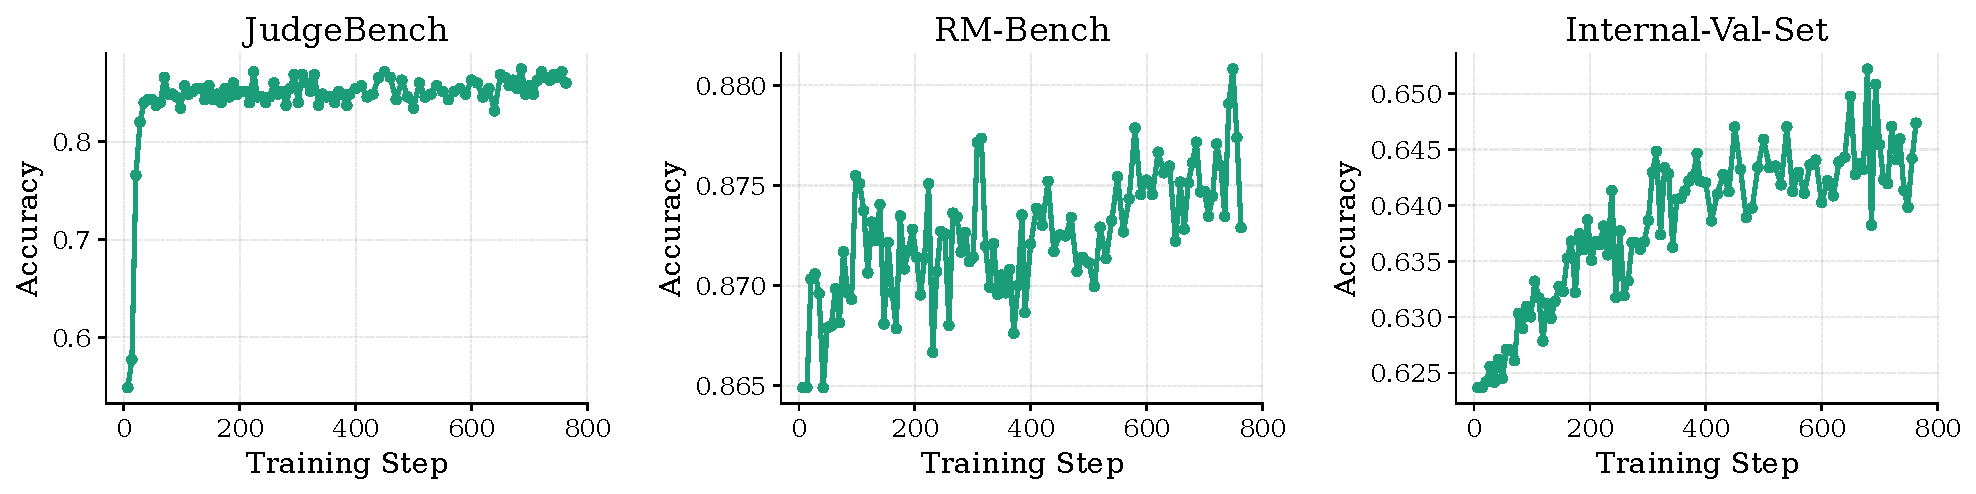
\includegraphics[width=\textwidth]{figures/genrm-training.pdf}
    \caption{GenRM performance improves across benchmarks as we scale up RL training.}
    \label{fig:genrm-training}
\end{figure}
\subsubsection{RLHF with Group Relative Length Control}
With a trained GenRM, we conduct RLHF on the same set of prompts. Same as RLVR, we use a batch of 128 prompts and 16 responses per prompt. Naively comparing all pairs of $N$ responses would require $\binom{N}{2}$ GenRM calls per prompt, which scales quadratically and becomes prohibitively expensive for large $N$. With $N=16$ responses, this would require 120 comparisons per prompt. Instead, we adopt a circular comparison strategy where each response is compared only with its successor: $(r_1, r_2), (r_2, r_3), \ldots, (r_{N-1}, r_N), (r_N, r_1)$, yielding exactly $N$ comparisons. This reduces computational cost from $O(N^2)$ to $O(N)$ while still connecting all responses in a comparison graph. Each response is also judged twice in different positions so as to alleviate positional bias.

For each pairwise comparison $(r_i, r_j)$, the GenRM produces individual helpfulness scores $s_i, s_j \in [1, 5]$ and a ranking score $s_r \in [1, 6]$. In the case where $s_i=s_j$, we further employ a simple tiebreaker mechanism:

\begin{align}
   s_i=s_i+(3.5-s_r), \\
   s_j = s_j + (s_r-3.5).
\end{align}

The base reward $R_i^{(\text{base})}$ for response $r_i$ is then computed by averaging its scores from two matches.

When training with base reward, we find that the length of response can rapidly increase as RLHF training proceeds. This is different from reward hacking, as the increase of length mostly comes from reasoning trace while only final answer is judged by GenRM. It is similar to observations in \citet{deepseekai2025deepseekr1incentivizingreasoningcapability} where model spends more inference time compute to achieve better rewards. However, unlike reasoning heavy tasks like math and coding, prompts in RLHF datasets usually don't require extensive reasoning. In order to reduce redundant thinking, we propose a Group Relative Length Control mechanism during RLHF. Specifically, for each prompt, we generate a group of $N$ candidate responses $\{r_1, r_2, \ldots, r_N\}$. Each response $r_i$ is decomposed into a reasoning component $r_i^{(\text{think})}$ and an answer component $r_i^{(\text{answer})}$, with corresponding lengths $\ell_i^{(\text{think})}$ and $\ell_i^{(\text{answer})}$.



\paragraph{Length-Normalized Reward Adjustment.} We compute a zero-mean, group-relative length bonus that encourages shorter responses within a group. For the reasoning component, we first normalize lengths within the group
\begin{align}
    w_i^{(\text{think})} = 1 - \frac{\ell_i^{(\text{think})} - \ell_{\min}^{(\text{think})}}{\ell_{\max}^{(\text{think})} - \ell_{\min}^{(\text{think})}},
\end{align}

where $\ell_{\min}^{(\text{think})} = \min_j \ell_j^{(\text{think})}$ and $\ell_{\max}^{(\text{think})} = \max_j \ell_j^{(\text{think})}$. To ensure the adjustment is zero-sum across the group (preserving the overall reward scale), we center the weights
\begin{align}
    \tilde{w}_i^{(\text{think})} = w_i^{(\text{think})} - \frac{1}{N}\sum_{j=1}^{N} w_j^{(\text{think})}.
\end{align}

The same procedure is applied to answer lengths to obtain $\tilde{w}_i^{(\text{answer})}$. The final reward for response $r_i$ is then
\begin{align}
    R_i = R_i^{(\text{base})} + \lambda^{(\text{think})} \tilde{w}_i^{(\text{think})} + \lambda^{(\text{answer})} \tilde{w}_i^{(\text{answer})},
\end{align}

where $R_i^{(\text{base})}$ is the base reward from pairwise comparisons and $\lambda^{(\text{think})}, \lambda^{(\text{answer})}$ are  coefficients controlling the strength of the length penalty. We set $\lambda^{(\text{think})}=0.5$, $\lambda^{(\text{answer})}=0.5$.
\paragraph{Quality-Gated Conciseness Bonus.} To further encourage concise responses without sacrificing quality, we introduce optional bonuses for the shortest responses that achieve top-tier quality scores. Let $\tau_p$ denote the $p$-th percentile threshold of scores within the group. For the response $r_k$ with minimum reasoning length:
$$R_k \leftarrow R_k + \beta^{(\text{think})} \cdot \mathbb{1}\left[R_k^{(\text{base})} \geq \tau_p\right]$$
Similarly, for the response $r_m$ with minimum answer length:
$$R_m \leftarrow R_m + \beta^{(\text{answer})} \cdot \mathbb{1}\left[R_m^{(\text{base})} \geq \tau_p\right]$$
where $\beta^{(\text{think})}$ and $\beta^{(\text{answer})}$ are the reasoning and answer conciseness bonuses respectively, and $\mathbb{1}[\cdot]$ is the indicator function. We set $\beta^{(\text{think})}=0.5$, $\beta^{(\text{answer})}=0.5$, and $\tau_p=80$.

This mechanism ensures that (1) length penalties are relative within each prompt group rather than absolute, avoiding bias against inherently complex problems; and (2) conciseness bonuses are only awarded to high-quality responses, preventing the model from learning to produce short but low-quality answers. We observe that the verbosity level reduces 30\% during the training without sacrificing accuracy.


\subsection{Post-trained Model Evaluations}
\label{subsec:final_model_evals}

\subsubsection{Evaluation Benchmarks}

\begin{table*}[!htp]
\centering
\small
\setlength{\tabcolsep}{7pt}
\renewcommand{\arraystretch}{1.15}

\begin{tabular}{l|c c c }
\toprule
\textbf{Benchmark} & \textbf{N-3-Nano} & \textbf{Qwen3} & \textbf{GPT-OSS} \\
\midrule

\rowcolor{black!5}
\multicolumn{4}{l}{\textbf{General Knowledge}} \\
MMLU-Pro &  78.30 &  \textbf{80.90} & 75.00 \\

\midrule
\rowcolor{black!5}
\multicolumn{4}{l}{\textbf{Reasoning}} \\
AIME25 (no tools) & 89.06 & 85.00 & \textbf{91.70} \\
AIME25 (with tools) & \textbf{99.17} & - & 98.7 \\
GPQA (no tools) &  73.04 & \textbf{73.40} & 71.50 \\
GPQA (with tools) & \textbf{75.00} & - & 74.20 \\
% LiveCodeBench (v5 2024-07$\leftrightarrow$12) & 72.063 & 66.000 & 78 \\
LiveCodeBench (v6 2024-08$\leftrightarrow$2025-05) & \textbf{68.25} & 66.00 & 61.00\\
SciCode (subtask) & 33.28 & 33.00 & \textbf{34.00}  \\
HLE (no tools) & 10.57 & 9.80 & \textbf{10.90} \\
HLE (with tools) & 15.48 & - & \textbf{17.30} \\
MiniF2F pass@1 & \textbf{50.03} & 5.72* & 12.05* \\
MiniF2F pass@32 & \textbf{79.92} & 16.80* & 43.03* \\
\midrule
\rowcolor{black!5}
\multicolumn{4}{l}{\textbf{Agentic}} \\
Terminal Bench (hard subset) & 8.51 & 5.00 & \textbf{10.00} \\
% Terminal Bench (nv-internal mix) &  &  &  \\
% SWE-Bench Verified & 38.760 & ? & 38.760 \\
SWE-Bench (OpenHands) & \textbf{38.76} & 22.00* & 34.00* \\
\textbf{TauBench V2} &  &  &  \\
\quad Airline & 48.00 & \textbf{58.00} & 38.00 \\
\quad Retail & 56.91 & \textbf{58.80} & 54.80 \\
\quad Telecom & 42.21 & 26.30 & \textbf{49.70} \\
\quad Average & \textbf{49.04} & 47.70 & 47.50 \\
% Aider-Polyglot &  &  &  \\
BFCL v4 & \textbf{53.76} & 46.40* & - \\
\midrule
\rowcolor{black!5}
\multicolumn{4}{l}{\textbf{Chat \& Instruction Following}} \\
IFBench (prompt) & \textbf{71.51} & 51.00 & 65.00 \\
% IFBench (instruction) & 77.015 &  &  \\
Scale AI Multi Challenge & 38.45  & \textbf{44.75} & 33.75 \\
Arena-Hard-V2 (Hard Prompt) & \textbf{72.10} & 49.60* & 71.20* \\
Arena-Hard-V2 (Creative Writing) & 63.20 &  \textbf{66.00*} & 25.90* \\
Arena-Hard-V2 (Average) & \textbf{67.65} & 57.80 & 48.55 \\

\midrule
\rowcolor{black!5}
\multicolumn{4}{l}{\textbf{Long Context}} \\
AA-LCR & 35.85 & \textbf{59.00} & 34.00 \\
RULER-100 @ 256k & \textbf{92.92} & 89.40 & - \\
RULER-100 @ 512K & \textbf{91.25} & 84.00 & - \\
RULER-100 @ 1M & \textbf{86.34} & 77.50 & - \\

\midrule
\rowcolor{black!5}
\multicolumn{4}{l}{\textbf{Multilingual}} \\
MMLU-ProX (avg over langs) & 59.50 & \textbf{77.60*} & 69.10* \\
% MMLU-ProX (avg over langs w/o Ja) &  &  &  \\
WMT24++ (en$\rightarrow$xx) & \textbf{86.20} & 85.60 & 83.20 \\
% COMET?? & &  &  \\

\bottomrule
\end{tabular}

\caption{
\ourmodel compared to \text{Qwen3-30B-A3B-Thinking-2507}, and \text{GPT-OSS 20B}. 
% \todo{JK: Structured Output environment} 
% \today{Alex: Genselect \& Formal proofs}
% \todo{Change precision to 1 decimal. There seems to be a discrepancy rn}
}
\label{tab:nano_v3_comparison}
\end{table*}


We evaluate \ourmodel across a broad suite of established benchmarks spanning mathematical and
scientific reasoning, coding, agentic tool use, instruction following, long-context understanding, and
multilingual capability. Table~\ref{tab:nano_v3_comparison} summarizes the final results.

All evaluation results were collected via Nemo Evaluator SDK\footnote{\url{https://github.com/NVIDIA-NeMo/Evaluator}} and for most benchmarks, the Nemo Skills Harness\footnote{\url{https://github.com/NVIDIA-NeMo/Skills}}. For reproducibility purposes, the open source container on Nemo Skills packaged via NVIDIA's Nemo Evaluator SDK used for evaluations can be found here\footnote{\url{https://catalog.ngc.nvidia.com/orgs/nvidia/teams/eval-factory/containers/nemo_skills}}. In addition to Nemo Skills, the evaluations also used dedicated packaged containers for Tau-2 Bench, ArenaHard v2, AA\_LCR. More details on the evaluation settings can be found in the Nemo Evaluator SDK configs folder\footnote{\url{https://github.com/NVIDIA-NeMo/Evaluator}}. The following benchmarks are not onboarded yet in our open source tools and for these we used their official open source implementation: Terminal Bench, SWE-Bench, Scale AI Multi Challenge.


For mathematical and STEM reasoning, we evaluate on \textsc{AIME25} (with and without tools), \textsc{GPQA}~\citep{rein2023gpqa}, \textsc{LiveCodeBench v6}~\citep{jain2024livecodebench},
\textsc{SciCode}~\citep{tian2024scicoderesearchcodingbenchmark},
and \textsc{Humanity’s Last Exam}~\citep{phan2025humanitysexam}.
We additionally include \textsc{MMLU-Pro} to assess general academic and
knowledge-intensive reasoning.

Agentic and tool-augmented capabilities are measured using \textsc{TerminalBench},
\textsc{SWE-Bench} (OpenHands) \citep{jimenez2023swe, wang2025openhandsopenplatformai}, 
\textsc{TauBench V2} (airline, retail, telecom) \citep{barres2025tau}, 
and \textsc{BFCL v4} \citep{patil2025bfcl}, each of which provides verifiable reward signals via
unit tests, database state transitions, or structured schema constraints.

Instruction-following and conversational ability are evaluated with \textsc{IFBench},
\textsc{Scale AI Multi-Challenge}, and \textsc{Arena-Hard-V2} \citep{li2024crowdsourced}. 
These benchmarks probe multi-constraint instructions, preference-aligned chat behavior, and faithfulness to user intent. For \textsc{Arena-Hard-V2}, we follow \citet{yang2025qwen3technicalreport} and use GPT-4.1 as judge.

Long-context performance is assessed with \textsc{RULER-100} at 256k, 512k, and 1M tokens \citep{hsieh2024ruler},
together with \textsc{AA-LCR}, evaluating retrieval, stability, and chain-of-thought
coherence over extreme context lengths. RULER-100 is evaluated with reasoning off, whereas AA-LCR is measured with reasoning on.

For multilingual capability, we report results on \textsc{MMLU-ProX} \citep{xuan2025mmlu} and
\textsc{WMT24++} (en$\rightarrow$xx) \citep{deutsch2025wmt24++}, covering a mix of reasoning and translation
settings across multiple high-resource languages.

For comparison with \textsc{GPT-OSS 20B} and \textsc{Qwen3-30B-A3B-Thinking-2507}, we use the officially reported numbers whenever available; if a benchmark is not reported, we take the value from ArtificialAnalysis (AA)\footnote{\url{https://artificialanalysis.ai/}}; and if neither source provides results, we may compute the scores ourselves using the official evaluation protocol.


Table \ref{tab:nano_v3_comparison} presents a comprehensive performance comparison between the three models. \ourmodel shows strong results, surpassing both GPT-OSS 20B and Qwen3-30B-A3B-Thinking-2507 in all categories. On reasoning benchmarks \ourmodel surpasses the Qwen3 model and is competitive with GPT-OSS, which was the previous best model in these categories. In the agentic, chat, and long context categories \ourmodel significantly outperforms both of the other models, demonstrating the strength of our post-training pipeline.
% \todo{eval with tool: is it only python tool?} \\
% \todo{ LCBv6 and LCB range. For now taking published numbers for qwen-3 and gpt-oss} \\
% \todo{Soumye: Model results over stages table on a subset of benchmarks}
% \todo{Key Findings where we put ablations}
% \begin{itemize}
%     \item MoEs beneift from more epochs (in SFT)
%     \item SFT initizlation 5k vs 13k vs 18k
% \end{itemize}



